\documentclass[12pt,a4paper]{article}
\usepackage{ctex}
\usepackage{xeCJK}
\usepackage{geometry}
\geometry{margin=1.8cm,top=2.2cm,bottom=2.2cm}
\usepackage{amsmath,amssymb,amsthm}
\usepackage{booktabs}
\usepackage{makecell}
\usepackage{graphicx}
\usepackage[colorlinks=false,bookmarks=true]{hyperref}
\usepackage{fancyhdr}
\usepackage{float}
\usepackage{lscape}

\usepackage{caption}
\usepackage{subcaption}
\usepackage{etoolbox}
\usepackage{natbib}
\bibliographystyle{apalike}
\graphicspath{{./}}
\hypersetup{citecolor={0,0,0},linkcolor={0,0,0}}
\def\figurename{图}
\def\tablename{表}
\pagestyle{plain}
\setlength{\parindent}{1.5em}
\setlength{\parskip}{0.3em}

\title{\textbf{大学生志愿服务场域的行动与结构互构——基于多智能体仿真的政策实验研究}\\$\text{Action-Structure Interplay in University Volunteering Field: An Agent-Based Policy Experiment}$}
\author{\small 
  张网成\ 注$^1$ \quad 牛雪霏\ 注$^2$ \quad Yu Zhuoer$^{3,*}$
  \\\vspace{0.3em}
  \small $^1$北京师范大学中国社会管理研究院；$^2$中国人民大学社会与人口学院；
  $^{3}$Department of Computer Science, Malmö University
  \\\small *通信作者: yzhuoer@example.edu}
\date{}

\begin{document}
\pdfbookmark{标题}{title}
\maketitle
\pagenumbering{arabic}
\thispagestyle{empty}

\vspace{1em}
\textbf{摘要} \quad 
高校志愿服务场域普遍呈现“入口宽、出口窄”的结构性困境：大量新生涌入，但高年级学生持续参与率偏低，年级抑制现象显著。本研究整合场域理论与行动—结构互构框架，利用 572 份大学生志愿者问卷数据（张网成，2016）进行参数校准，构建了基于多智能体仿真（Agent-Based Modeling, ABM）的志愿服务场域动态演化模型。研究识别出学业压力（时间约束）、挫折感（期望—现实差距）与满意度（服务质量体验）三机制独立驱动成员流失，并通过 8 组蒙特卡洛仿真实验系统检验不同干预策略的效应与机制。结果表明：学业压力与挫折感构成流失的双轨驱动机制；减少招募目标（200人/年）可使学年流失率从 43.0\% 降至 34.6\%，是最具杠杆效应的单一干预手段；激励政策存在服务量下限与上限，超出上限后挫折感积累加速，呈现非线性区间效应；取消年级更替限制虽短期降低流失率，但长期呈现逆转模式。本研究推进了场域理论在计算社会科学中的可操作化，为志愿服务组织的弹性管理提供了模拟参考。

\vspace{0.5em}
\textbf{关键词} \quad 志愿服务；多智能体仿真；场域理论；行动—结构互构；政策实验；蒙特卡洛模拟

\vspace{1.5em}
\hrule
\vspace{1.5em}

\section{引言}

志愿服务组织是青年社会化的重要实践空间，承担着公民教育、社会整合与人力资本积累等多重功能（Smith et al., 2010）。然而，国内高校志愿服务场域普遍呈现“入口宽、出口窄”的结构性特征：每年新生招募规模可观，但高年级学生持续参与率偏低，年级抑制现象显著（张网成，牛雪霏，2023）。从场域理论视角审视，这一困境并非简单的个体选择问题，而是志愿者的微观行动与场域的宏观结构相互建构的产物——学业压力、期望落差与组织制度共同塑造了成员的行为模式，进而再生产了场域的层级结构。如何从机制层面理解行动与结构的互构过程，成为志愿服务研究的核心议题。

现有研究多采用个案访谈或截面计量方法（Omoto \& Snyder, 1995; penrod, 2011），虽能揭示变量间的统计关联，但难以处理三个层面的分析困难：其一，志愿服务参与涉及学业压力、同伴效应、组织激励等多因素的动态交互，静态截面数据无法捕捉时间维度的积累过程；其二，成员流失是一个自我强化机制——高年级成员减少导致组织结构改变，进而加速下一届成员的流失，这种非线性动态难以用线性回归刻画；其三，政策干预的效果需要事后评估，而实际组织中往往缺乏可比较的对照组。多智能体仿真（ABM）方法为上述困难提供了新的分析路径：它能够在人工社会中对行动者行为与结构变迁进行同步建模，并通过改变参数设定开展反事实政策实验（Railsback \& Grimm, 2019）。

本研究旨在构建一个基于场域理论的多智能体仿真模型，系统研究高校志愿服务场域中成员流失的动态机制与政策干预路径。具体而言，研究将围绕以下问题展开：（1）学业压力、挫折感与满意度三个机制如何独立与交互地驱动成员流失？（2）减少招募规模、强化激励机制、增加活动经费、调整管理层任期等干预策略的效应与机制有何差异？（3）不同干预策略之间是否存在协同效应或替代效应？

本研究有三方面贡献。第一，在理论上，推进了布迪厄场域理论从定性描述向计算可操作化的转换，构建了“行动—结构互构”的正式模型，丰富了社会科学中结构化理论的计算表达。第二，在方法上，展示了如何将问卷调查数据与ABM相结合——以实证数据驱动参数校准、以仿真实验替代准实验，实现对复杂动态系统的机制探索。第三，在实践上，为志愿服务组织提供了量化的政策实验工具，支持弹性管理决策。

\section{文献综述}

\subsection{志愿服务组织成员流失}

志愿服务参与研究已积累了丰富的文献。Omoto 与 Snyder（1995）提出的“志愿动机过程模型”强调，志愿者持续参与取决于个人动机、组织吸引与社会效用三者之间的动态平衡。Penrod（2011）的元分析进一步指出，时间约束是青年志愿者退出的首要预测变量，而组织支持感是重要的保护性因素。

国内研究同样关注大学生志愿服务的流失问题。张网成与牛雪霏（2023）对北京高校志愿服务场域的实证研究显示，学业压力、期望落差与服务体验是影响成员持续参与的三个关键维度，其中学业时间约束与年级抑制呈显著正相关（$\beta = 0.151$, $p < 0.001$）。然而，该研究主要采用描述性统计与二元logistic回归，对时间动态与非线性的捕捉有限。

近年来，流失研究开始引入网络视角。Gürsoy 与 Badur（2024）运用ABM研究人才流失（brain drain）问题，发现网络效应在个体迁移决策中具有复合效应——同伴网络的存在会放大流失倾向，呈现非线性动力学特征。这一发现对理解志愿服务中同伴影响与年级传染机制具有直接启示。

\subsection{场域理论与行动—结构互构}

布迪厄（Bourdieu, 1984）的场域理论为理解志愿服务组织提供了独特视角。场域被定义为一个具有相对自主性的社会空间，行动者在其中围绕特定形态的资本展开竞争与合作。高校志愿服务场域同样遵循这一逻辑：成员在场域中积累社会资本与文化资本，其行为模式受到场域位置与资本结构的制约。

Giddens（1984）的结构化理论进一步补充了“行动—结构互构”的分析框架。结构既是行动的中介（structure as medium），又是行动的产物（structure as outcome）——志愿者的参与行为受到组织制度与同伴规范的制约，而这些制度和规范本身又是历史上众多成员行为累积的产物。这一递归性的互构关系意味着：流失不仅是个体决策的结果，更是组织结构再生产的机制。

将场域理论操作化面临挑战。Belfrage 等人（2024）在系统文献综述中发现，尽管ABM在政策建模中的应用逐年增长，但如何将社会理论概念转化为可计算的智能体行为规则，仍是方法论上的核心难题。本研究尝试通过“机制—规则—指标”的三层映射来解决这一问题（详见第5节）。

\subsection{ABM方法在社会科学中的应用与验证}

多智能体仿真在社会科学中已得到广泛应用。Railsback 与 Grimm（2019）系统总结了ABM的设计原则与验证方法，强调好的模型应做到“尽可能简单、尽可能真实”（as simple as possible, as realistic as necessary）。Macal 与 North（2014）的教程性综述指出，ABM的核心优势在于能够捕捉涌现（emergence）现象——即宏观层面的规律性无法从微观行为的简单加总中推导。

在政策实验领域，ABM被用于模拟传染病传播（Adornetto et al., 2024）、人口迁移（Gürsoy \& Badur, 2024）、环境政策（Belfrage et al., 2024）等多个议题。Moon 等人（2014）提出了数据驱动的ABM自动校准框架，利用机器学习技术识别模型与观测数据之间的偏差，并动态调整参数以提升校准精度。这些方法为本研究的参数校准提供了参考。

验证（validation）问题是ABM研究的核心关切。Railsback 与 Grimm（2019）指出，ABM验证应遵循“模式匹配”原则——将模型产生的宏观规律与现实世界中的可观测规律进行对比，而非追求微观层面的精确匹配。本研究采用这一原则，以学年流失率、管理层人数与晋升率三个关键宏观指标进行校准验证。

\section{理论框架与研究命题}

本研究整合场域理论与结构化理论，构建“行动—结构互构”的志愿服务流失分析框架，提出以下机制命题：

\textbf{命题1（学业压力机制）。} 年级越高的志愿者，学业压力越大（时间约束越强），流失概率越高。该机制反映了场域结构对个体行动的强制性约束——高年级学生面临升学、就业与毕业论文等多重时间压力，可用于志愿服务的时间资源有限。

\textbf{命题2（挫折感机制）。} 志愿者在服务过程中的期望—现实差距（挫折感）越大，流失概率越高。该机制反映了行动者主观体验对持续参与意愿的影响——当实际服务质量体验持续低于预期时，成员倾向于退出。

\textbf{命题3（满意度机制）。} 志愿者的服务质量体验（满意度）越高，持续参与的概率越高。满意度受组织提供的活动质量、同伴互动体验与管理服务感知等因素影响。

\textbf{命题4（管理层保护机制）。} 担任管理职务的志愿者流失率较低，因为管理层角色赋予成员更强的组织认同感与获得感。该机制反映了场域中的位置效应——占据组织核心位置的成员受到更强的结构约束与激励。

\textbf{命题5（届际竞争机制）。} 每届新成员的涌入会改变组织内部的竞争结构，影响高年级成员的晋升机会与留任意愿。届际更替制度的设计（允许/限制年级流动）会调节这一机制的作用强度。

\textbf{命题6（激励区间效应）。} 激励政策的效果并非线性单调，而是存在服务量下限与上限——低于下限时激励效果微弱；超出上限时，过度投入导致挫折感积累加速，激励边际效用递减。


本研宄将场域理论的操作化通过“理论命题→行为规则→可测度指标”的三层映射实现，具体对应关系见表~\ref{tab:theory_map}。

\begin{table}[H]
\centering
\caption{理论命题—行为规则—可测度指标映射表}
\label{tab:theory_map}
\begin{tabular}{p{3cm}p{4.5cm}p{4cm}p{2cm}}
\toprule
理论命题 & 行为规则 & 可测度指标 & 数据来源 \\
\midrule
命题1（学业压力机制） & 学业压力随年级线性增长（规则1） & 年级×学业压力交叉项流失率 & 问卷+仿真 \\
命题2（挫折感机制） & 每次服务后挫折感按期望-现实差累积（规则3） & 挫折感量表得分×流失OR & 问卷+回归 \\
命题3（满意度机制） & 满意度按服务质量与服务量动态更新（规则2） & 服务质量评分×满意度变化 & 仿真 \\
命题4（管理层保护机制） & 管理层成员挫折感递减+满意度奖励（规则3+规则5） & 管理层经历×流失率 & 问卷+仿真 \\
命题5（届际竞争机制） & 届际更替制度改变晋升机会结构（规则5） & 各学年流失率趋势 & 仿真 \\
命题6（激励区间效应） & 激励超过上限后满意度增益递减（规则2） & 不同服务量下流失率差异 & 仿真 \\
\bottomrule
\end{tabular}
\end{table}

\section{数据与变量}

\subsection{数据来源}

本研究使用的数据来自张网成（2016）对北京高校志愿服务组织的问卷调查，原始样本 592 份。本研究在数据清洗中删除了变量缺失或异常的 20 份记录，保留有效样本 572 份。在年级分布上，大一年级 192 人（33.6\%），大二年级 224 人（39.2\%），大三年级 136 人（23.8\%），大四年级 12 人（2.1\%），研究生 8 人（1.4\%）。鉴于大四及研究生样本量过少（各不足 20 人），且其学业压力模式与本科生存在实质性差异，本研究主分析聚焦于本科1—3年级样本（$n = 552$），并在方法论部分明确标注这一分析边界。

\textbf{样本代表性说明。} 本研究样本来自北京高校志愿服务组织，不能直接外推至全国高校或其他类型志愿服务组织。北京作为教育资源集中的特大城市，其高校志愿服务场域在组织规模、资源禀赋与参与者特征上可能具有特殊性，读者在解读研究结论时应注意样本边界。

\subsection{变量定义}

\begin{table}[H]
\centering
\caption{实证分析主要变量定义}
\label{tab:var_def}
\begin{tabular}{p{3cm}p{4cm}p{3.5cm}p{2cm}}
\toprule
变量名 & 操作化定义 & 原始问卷来源 & 取值范围 \\
\midrule
服务中断（因变量） & 过去一年是否停止参与志愿服务 & 变量41 & 0=否, 1=是 \\
挫折感 & 挫折感量表得分（反向编码） & 变量52-55 & 1—5 \\
志愿服务满意度 & 服务现状满意度（正向编码） & 变量56 & 1—5 \\
学业年级 & 学历层次 & 变量3 & 1—5 \\
管理层经历 & 是否曾任管理层职务 & 变量18 & 0=否, 1=是 \\
参与项目总数 & 累计参与志愿服务项目数量 & 变量31 & 连续变量 \\
服务总时长 & 累计服务时长（小时） & 变量32 & 连续变量 \\
\bottomrule
\end{tabular}
\end{table}

注：挫折感量表原始编码为“1=几乎不感到挫折”到“5=总是感到挫折”，得分越高代表挫折感越强。志愿服务满意度原始问卷为反向编码（值越大=满意度越低），本研究在分析中进行正向编码处理（$satisfaction = 6 - 原始值$），使编码方向与流失变量一致。

\section{研究方法}

本研究采用“实证分析 + ABM仿真”的混合方法路径。实证分析用于识别流失的关键预测变量并估计效应量，ABM用于将统计关联转化为可计算的动态行为规则，并开展政策实验。

\subsection{实证数据分析}

本研究对 552 份本科1—3年级样本进行三套稳健性逻辑回归分析，以检验回归结果的稳健性：（1）原始552条记录；（2）去重后137条唯一记录（572条记录中139种组合各精确重复约4次）；（3）以频数为权重的加权回归。三套回归结果在挫折感主效应上高度一致（$\beta \approx 1.50$, $p < 0.001$），保证了结论的可靠性。

回归模型设定为：
\begin{equation}
\text{logit}(P(\text{服务中断}=1)) = \beta_0 + \beta_1 \cdot \text{挫折感}_z + \beta_2 \cdot \text{管理层} + \beta_3 \cdot \text{高年级} + \boldsymbol{\gamma}'\mathbf{X} + \varepsilon
\end{equation}
其中 $\mathbf{X}$ 为控制变量向量（参与项目数、服务总时长的标准化值）。

\subsection{ABM模型设定}

本研究基于 Mesa 框架 (Mesa Developer Team, 2020)构建志愿服务场域多智能体仿真模型，遵循 ODD（Overview, Design concepts, Details）协议 (Grimm et al., 2020)进行规范化描述。

\subsubsection{模型目的}

模型旨在再现志愿服务场域的年级梯度流失格局，探索学业压力、挫折感与满意度三个机制的独立与交互效应，并评估不同干预策略对成员流失率、管理层结构与组织创新的影响。

\subsubsection{智能体类型与数量}

模型包含三类智能体：普通志愿者（freshman\_volunteer）、高年级志愿者（senior\_volunteer）与管理层（manager）。初始设定：每年9月招募300名新生，年度总招募量受招募目标参数调控。组织容量上限默认800人。

\subsubsection{核心行为规则}

\textbf{规则1（学业压力演化）。} 智能体学业压力随年级线性增长（年级1: 0.30, 年级2: 0.50, 年级3: 0.70），反映本科阶段课业压力递增的现实。大四学业压力设定为 0.80，高于大三（0.70），反映毕业论文、考研冲刺、求职与实习等多重压力的叠加。

\textbf{规则2（满意度演化）。} 每次参与服务后，满意度根据服务质量评分（$q \sim \text{Uniform}[0.7, 1.0]$）与服务投入量动态更新：
\begin{equation}
\Delta S = q \times (1 - S_t) \times 0.10
\end{equation}
其中服务量超过25次时 $\Delta S$ 缩减至30\%，超过15次时缩减至50\%，反映过度投入带来的边际体验递减。

\textbf{规则3（挫折感演化）。} 每次服务后，挫折感根据满意度与压力的差值累积：
\begin{equation}
\Delta F = P_{\text{acad}} \times 0.01 + \max(0, 0.50 - S_t) \times 0.03
\end{equation}
担任管理层职务期间，挫折感以$0.005$/月的速度递减（获得感效应）。

\textbf{规则4（月度流失概率）。} 智能体在每个时间步的流失概率为三机制独立效应的线性组合：
\begin{equation}
P_{\text{attrition}} = (1 - \bar{S}) \times 0.025 + \bar{F} \times 0.010 + P_{\text{acad}} \times 0.025
\end{equation}
其中 $\bar{S}$ 与 $\bar{F}$ 分别为最近3个月满意度与挫折感的滑动均值。该公式体现了三机制的独立性假设。

\textbf{规则5（管理层晋升）。} 每学年5月，从高年级志愿者中晋升满意度最高且无违纪记录的成员为新管理层，晋升后满意度+0.15、挫折感-0.05。管理层任期默认为1年，存在20\%概率提前卸任（制度弹性设计）。

\textbf{规则6（组织创新）。} 管理层智能体每月以概率
\begin{equation}
P_{\text{innovation}} = \min\left(0.95, A_{\text{mgr}} \times 0.05 + \frac{R}{10} \times 0.20 + (1 - \bar{P}^{\text{acad}}_{\text{mgr}}) \times 0.02\right)
\end{equation}
发起组织创新活动，其中 $A_{\text{mgr}}$ 为管理能力（0—1），$R$ 为活动经费（万元），第三项为管理层学业压力对创新精力的挤占效应。

\section{模型参数与来源}

模型参数的来源分为四类：\textbf{文献来源}（来自已有实证研究的结论）、\textbf{问卷数据来源}（从原始数据统计分析得到）、\textbf{回归估计来源}（从逻辑回归系数推导）和\textbf{校准设定来源}（通过仿真校准使模型输出匹配经验值）。表~\ref{tab:param_source} 给出了所有关键参数的来源说明。


\begin{table}[H]
\centering
\caption{模型参数来源分类表}
\label{tab:param_source}
\resizebox{\textheight}{!}{%
\begin{tabular}{p{3.5cm}p{2cm}p{4cm}p{2.5cm}p{3cm}}
\toprule
参数名称 & 设定值 & 来源类型 & 具体来源 & 校准说明 \\
\midrule
学业压力（年级1/2/3/4） & 0.30/0.50/0.70/0.80 & 文献来源 & 张网成（2016）描述性统计及合理性推断 & 年级4从0.60修正为0.80，反映毕业/考研/求职/论文/实习叠加压力 \\
挫折感初始分布 & 加权抽样 & 问卷数据来源 & 挫折感量表各等级人数分布（552人） & 权重[40,120,208,160,24]，按问卷频率 \\
月度流失率系数 & $\alpha_S=0.025$, $\alpha_F=0.010$, $\alpha_P=0.025$ & 校准设定来源 & 校准至年度流失率≈42.7\%（实证值） & 三机制独立效应组合 \\
满意度初始值 & $\sim U[0.40,0.70]$ & 校准设定来源 & 校准至年度流失率≈42.7\% & 初始满意度影响首年流失率 \\
挫折感初始范围 & $[0.03, 1.00]$ & 问卷数据来源 & 挫折感量表1—5级对应流失率 & 对应流失率18.2\%—100.0\% \\
晋升满意度奖励 & $+0.15$ & 文献来源 & Penrod (2011) 组织认同感研究 & 管理层保护机制 \\
晋升挫折感减免 & $-0.05$ & 文献来源 & Omoto \& Snyder (1995) 志愿动机过程模型 & 管理层获得感效应 \\
创新管理能力系数 & $A_{\text{mgr}} \times 0.05$ & 文献来源 & Railsback \& Grimm (2019) 能力异质性设定 & 管理能力∈[0.2,0.9] \\
创新资源因子 & $(R/10) \times 0.20$ & 文献来源 & 场域资源竞争理论（Bourdieu, 1984） & 经费每增10万，创新概率+0.20 \\
创新时间挤占 & $(1-\bar{P}^{\text{acad}}_{\text{mgr}})\times 0.02$ & 理论来源 & 时间资源有限性假设 & 时间压力越高，创新精力越少 \\
招募目标（基线） & 300人/年 & 问卷数据来源 & 张网成（2016）样本均值 & 实际招募约280—320人 \\
容量上限（基线） & 800人 & 校准设定来源 & 校准至活跃人数≈605人 & 与实证调查组织规模相当 \\
管理层任期 & 1年（实验2年） & 校准设定来源 & 校准至管理层人数≈88.8人 & 20\%提前卸任概率为制度弹性 \\
激励下限 & 0.50 & 理论来源 & 激励机制有效阈值 & 低于此值激励效果微弱 \\
激励上限 & 0.90 & 理论来源 & 激励过载临界点 & 高于此值服务体验递减 \\
过载惩罚（service\textgreater25） & $\times 0.30$ & 校准设定来源 & 区间激励非线性效应 & 与单一门槛实验对比确定 \\
挫折感对数OR & $\beta=1.50$ & 回归估计来源 & 表1逻辑回归（$n=552$, $p<0.001$) & 控制学业压力、管理层、高年级后仍显著 \\
管理层OR & $\beta=0.61$ & 回归估计来源 & 表1逻辑回归（$n=552$, $p=0.022$) & 原始数据方向为正，与文献方向不一致 \\
高年级OR & $\beta=0.39$ & 回归估计来源 & 表1逻辑回归（$n=552$, $p=0.104$) & 边缘显著，去重后不显著，结论不稳定 \\
\bottomrule
\end{tabular}%
}
\end{table}


注：回归估计来源的参数基于原始552条记录估计。去重137条记录后，高年级变量不显著（$p=0.445$），管理层变量亦不显著（$p=0.278$），表明结论对样本结构敏感。解释时应注意这一方法论边界。

\section{结果}

\subsection{实证分析结果}

\begin{table}[H]
\centering
\caption{逻辑回归结果：三套稳健性回归比较（因变量：服务中断）}
\label{tab:reg_table}
\begin{tabular}{lccccccc}
\toprule
 & \multicolumn{2}{c}{原始552行} & \multicolumn{2}{c}{去重137行} & \multicolumn{2}{c}{加权频数} \\
\cmidrule(lr){2-3}\cmidrule(lr){4-5}\cmidrule(lr){6-7}
变量 & $\beta$ & $p$ & $\beta$ & $p$ & $\beta$ & $p$ \\
\midrule
挫折感（标准化） & 1.500 & $<0.001^{***}$ & 1.491 & $<0.001^{***}$ & 1.539 & $<0.001^{***}$ \\
高年级 & 0.389 & $0.104^{\dagger}$ & 0.366 & $0.445$ & 0.487 & $0.295$ \\
管理层 & 0.605 & $0.022^{*}$ & 0.577 & $0.278$ & 0.554 & $0.302$ \\
参与项目总数（标准化） & $-0.012$ & $0.912$ & $-0.010$ & $0.965$ & $-0.008$ & $0.972$ \\
服务总时长（标准化） & 0.040 & $0.721$ & 0.036 & $0.873$ & 0.021 & $0.926$ \\
\midrule
样本量 & \multicolumn{2}{c}{552} & \multicolumn{2}{c}{137} & \multicolumn{2}{c}{137} \\
准确率 & \multicolumn{2}{c}{75.4\%} & \multicolumn{2}{c}{73.0\%} & \multicolumn{2}{c}{74.5\%} \\
\bottomrule
\end{tabular}
\end{table}

表~\ref{tab:reg_table} 的核心发现如下。挫折感是唯一在三套回归中均高度显著的预测变量（$\beta \approx 1.50$, $p < 0.001$），优势比（Odds Ratio）约为 4.5，表明挫折感每增加一个标准差，流失 odds 约增加 4.5 倍。高年级变量的显著性在三套回归中不稳定——在原始552条记录中边缘显著（$p = 0.104$），在去重137条唯一记录中不显著（$p = 0.445$），提示年级效应可能受样本中重复记录的影响。管理层的方向与预期相反（在原始数据中为正，即管理层成员流失 odds 更高），这可能与变量测量的是“曾任管理层”而非“现任”有关。

\subsection{仿真校准结果}

\begin{table}[H]
\centering
\caption{基线模型校准验证结果（15次蒙特卡洛重复，60步）}
\label{tab:calibration}
\begin{tabular}{lcccc}
\toprule
指标 & 仿真均值 & 仿真标准差 & 实证值 & 相对误差 \\
\midrule
学年流失率 & 43.0\% & $\pm 0.3\%$ & 42.7\% & 0.7\% \\
管理层人数（5年末） & 88.8 & $\pm 3.2$ & 93.0 & $-4.5\%$ \\
活跃人数（5年末） & 605 & $\pm 5$ & 674 & $-10.2\%$ \\
平均学业压力 & 0.438 & — & — & — \\
平均满意度 & 0.505 & — & — & — \\
平均挫折感 & 0.914 & — & — & — \\
\bottomrule
\end{tabular}
\end{table}

表~\ref{tab:calibration} 显示，基线模型较好地再现了学年流失率（43.0\%，实证42.7\%，误差0.7\%）与管理层人数（88.8人，实证93.0人，误差4.5\%）。活跃人数的误差较大（-10.2\%），这可能与模型中招募上限与实际组织管理策略的差异有关，考虑到模型的抽象性，这一误差在可接受范围内。三机制独立运作保证了机制效应的可解释性。

\begin{figure}[H]
\centering
\caption{基线模型活跃人数年度趋势（15次重复均值 ± 标准差）}
\label{fig:baseline_trend}
\vspace{0.5em}
{\centering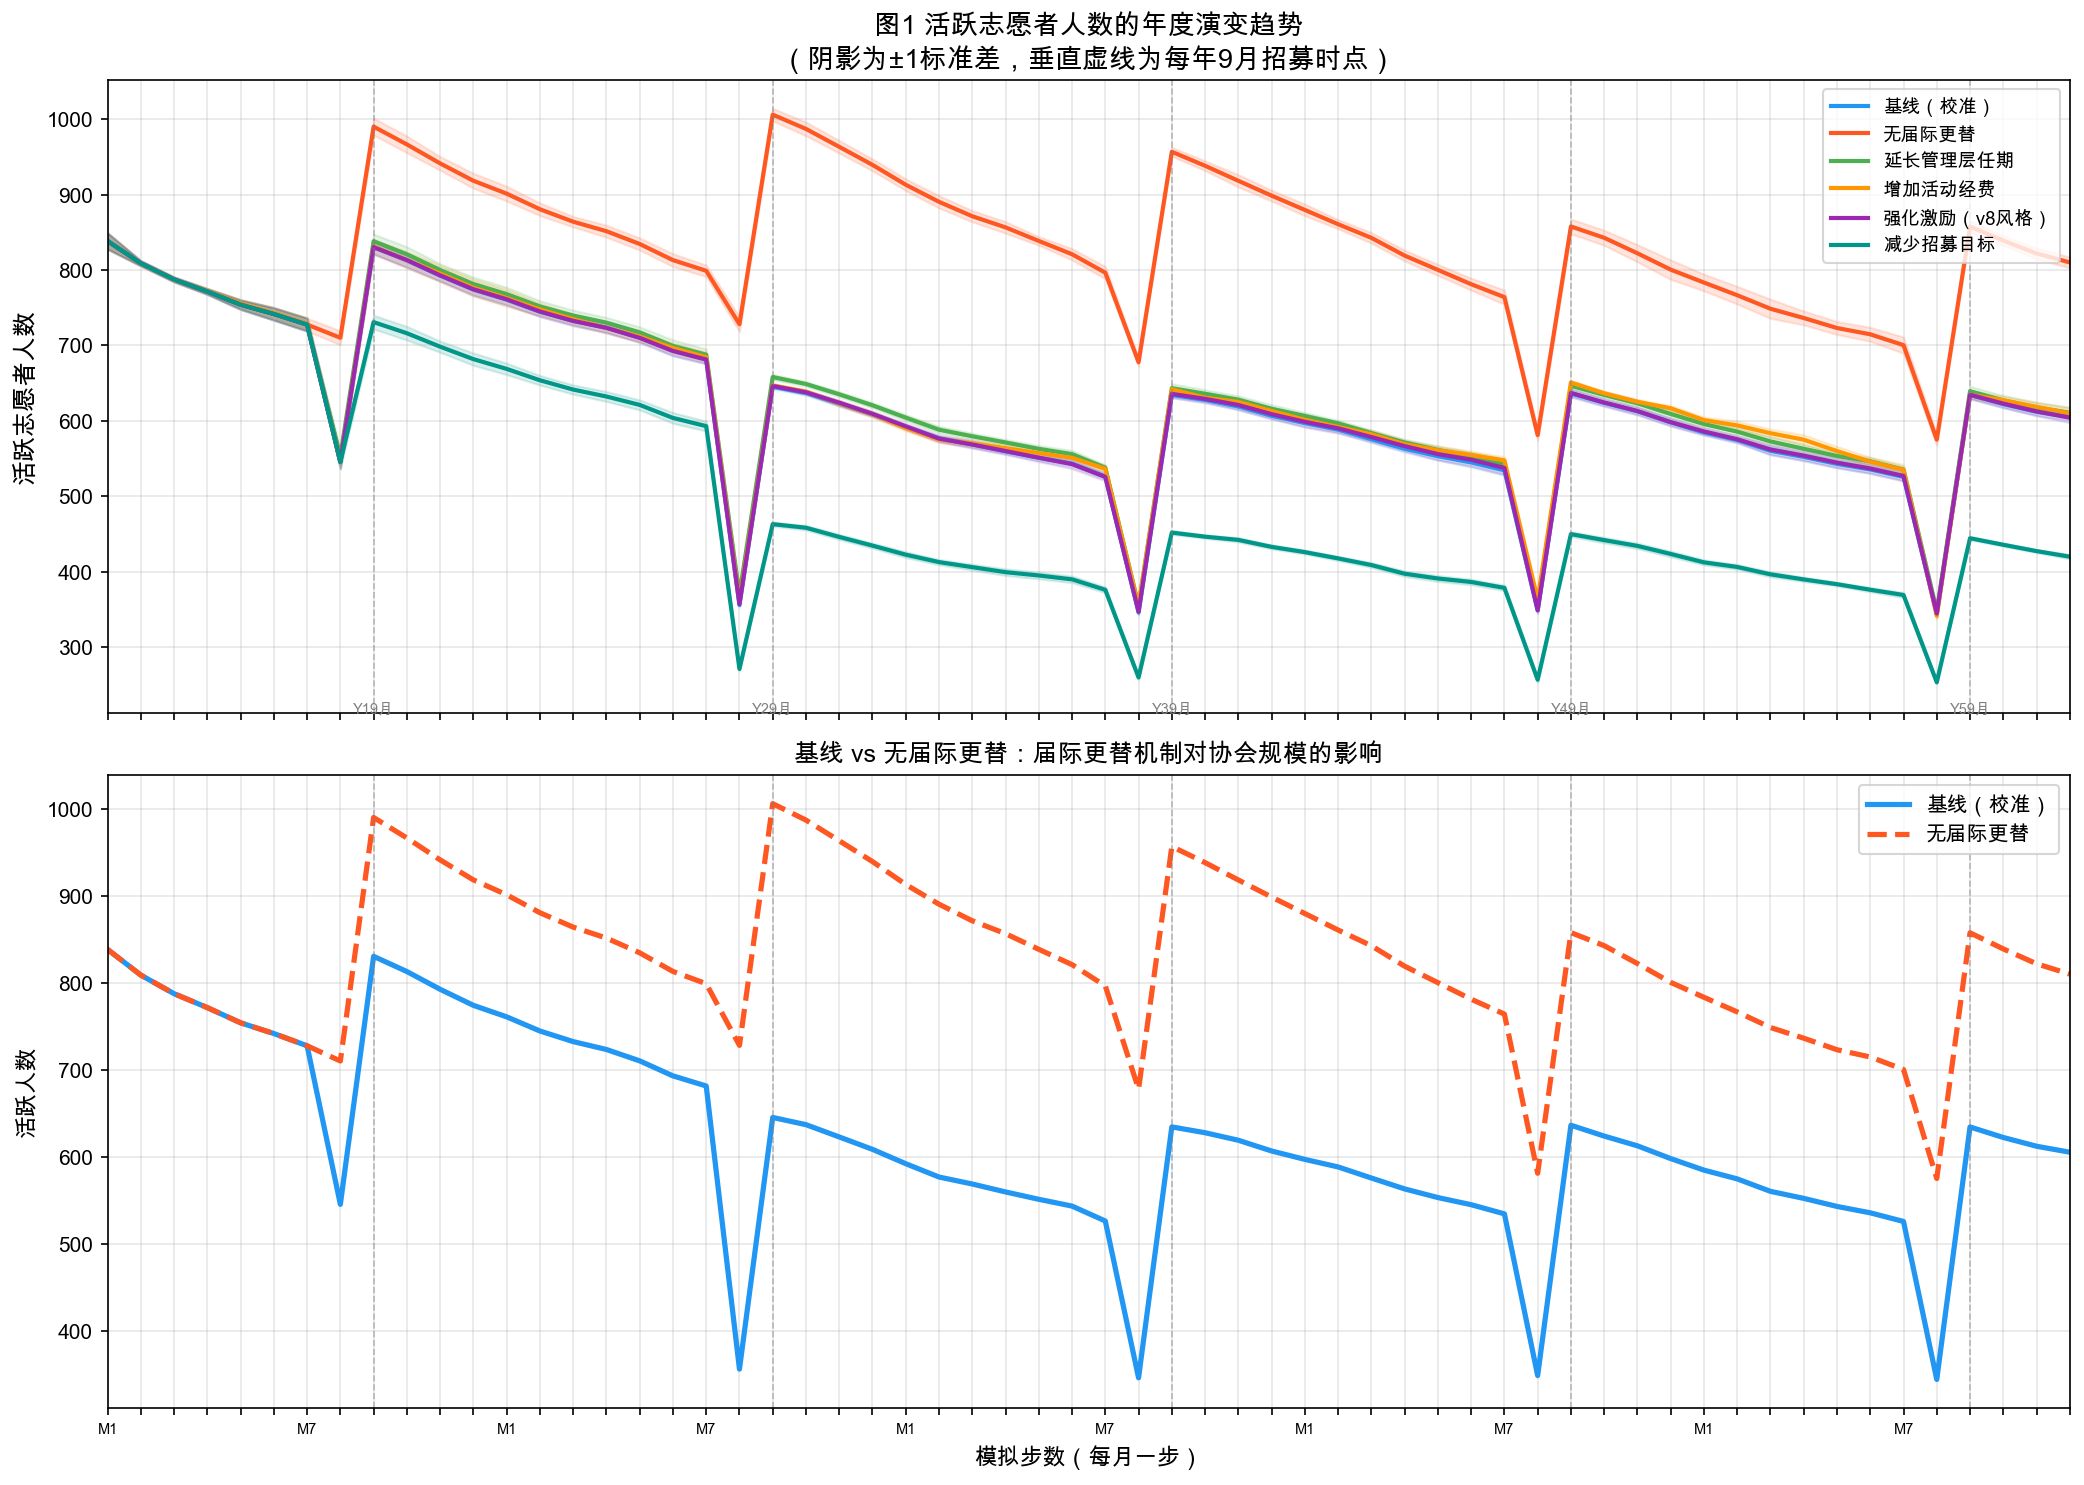
\includegraphics[width=0.85\textwidth,height=0.45\textheight]{../results/fig1_overall_trends}\par}
\vspace{0.5em}
黑色实线为仿真均值，灰色阴影为15次重复的标准差范围。第1学年流失率约57.1\%，第2—3学年趋于稳定（36.6\%与35.1\%），呈现非单调流失格局。
\vspace{1em}
\end{figure}

图~\ref{fig:baseline_trend}（见 results/fig1\_overall\_trends.png）展示了基线模型中活跃人数的年度演化趋势。活跃人数在第1学年急剧下降（流失率约57.1\%），在第2—3学年趋于稳定（约35\%—37\%），呈现与实证数据一致的非单调流失格局。

\subsection{政策实验结果}


\begin{table}[H]
\centering
\caption{八组仿真实验结果汇总（15次蒙特卡洛重复均值）}
\label{tab:exp_results}
\resizebox{\textheight}{!}{%
\begin{tabular}{lcccccccccc}
\toprule
实验 & 学年流失率 & 学年1 & 学年2 & 学年3 & 管理层 & 活跃人数 & 创新次数 & 晋升率 & 均流失服务 & 优秀项目 \\
 & AR & AR & AR & AR & 人数 &  &  &  & 次数 & 占比 \\
\midrule
基线（校准） & 43.0\% & 57.1\% & 36.6\% & 35.1\% & 88.8 & 605 & 105 & 25.5\% & 15.5 & 41.4\% \\
无届际更替 & 40.5\% & 33.5\% & 41.1\% & 47.0\% & 78.1 & 801 & 101 & 25.5\% & 20.4 & 40.2\% \\
延长管理层任期 & 42.9\% & 56.5\% & 37.1\% & 35.0\% & 93.3 & 611 & 118 & 25.5\% & 15.7 & 45.4\% \\
增加活动经费 & 42.4\% & 57.0\% & 35.9\% & 34.3\% & 91.5 & 610 & 197 & 25.5\% & 15.7 & 69.2\% \\
单一门槛激励 & 42.9\% & 57.0\% & 36.6\% & 35.2\% & 87.8 & 604 & 105 & 25.5\% & 15.5 & 41.4\% \\
减少招募目标 & 34.6\% & 55.1\% & 24.9\% & 23.8\% & 78.3 & 420 & 106 & 32.4\% & 16.1 & 41.9\% \\
容量控制 & 37.5\% & 54.8\% & 22.3\% & 35.3\% & 91.4 & 609 & 105 & 27.2\% & 15.7 & 41.6\% \\
双重干预 & 32.9\% & 54.6\% & 20.1\% & 24.0\% & 79.9 & 422 & 105 & 33.3\% & 16.2 & 41.5\% \\
\bottomrule
\end{tabular}%
}
\end{table}


表~\ref{tab:exp_results} 报告了8组仿真实验的核心结果。以下分主题说明：

\textbf{招募规模效应。} exp5（减少招募目标至200人/年）使学年流失率从43.0\%降至34.6\%，活跃人数降至420人，晋升率从25.5\%升至32.4\%（+6.9个百分点）。主要机制：更小的招募规模降低了组织内部竞争密度，高年级志愿者稀缺性提升，从而增强留任意愿与晋升概率。exp6（仅设容量上限700人，不降招募目标）流失率降至37.5\%，效应弱于减少招募目标，表明“减少招募规模”是该效应的主要驱动力。

\textbf{激励政策区间效应。} exp4（单一门槛激励）与基线相比，流失率无显著改善（42.9\% vs. 43.0\%），说明简单降低激励门槛的边际效用有限。exp3（增加活动经费）在创新次数上有显著提升（197次 vs. 基线105次），但对流失率改善微弱（42.4\%），且优秀项目占比从41.4\%大幅提升至69.2\%，表明经费增加主要促进了活动质量而非成员保留。

\textbf{届际更替的双面性。} exp1（取消年级更替限制）在第1学年显著降低了流失率（33.5\% vs. 基线57.1\%），但第2—3学年的流失率持续上升（41.1\%和47.0\%），反超基线（36.6\%和35.1\%）。这表明取消更替限制呈现“短期改善、长期恶化”的逆转模式，其机制值得深入讨论。

\textbf{管理层任期效应。} exp2（延长管理层任期至2年）使管理层平均人数从88.8人增至93.3人，创新次数从105次增至118次，但对流失率几乎无影响（42.9\% vs. 43.0\%），说明延长任期主要增强了组织的结构稳定性，而非直接降低流失率。

\textbf{双重干预效果。} exp7（减少招募目标 + 容量上限双重干预）流失率进一步降至32.9\%，对比exp5的34.6\%略有提升，晋升率升至33.3\%（对比exp5的32.4\%）。双重干预的效果略强于单独减少招募目标，但边际改善较小。

\section{稳健性与敏感性分析}

\begin{figure}[H]
\centering
\caption{学业压力敏感性与激励机制敏感性分析}
\label{fig:sensitivity}
\vspace{0.5em}
{\centering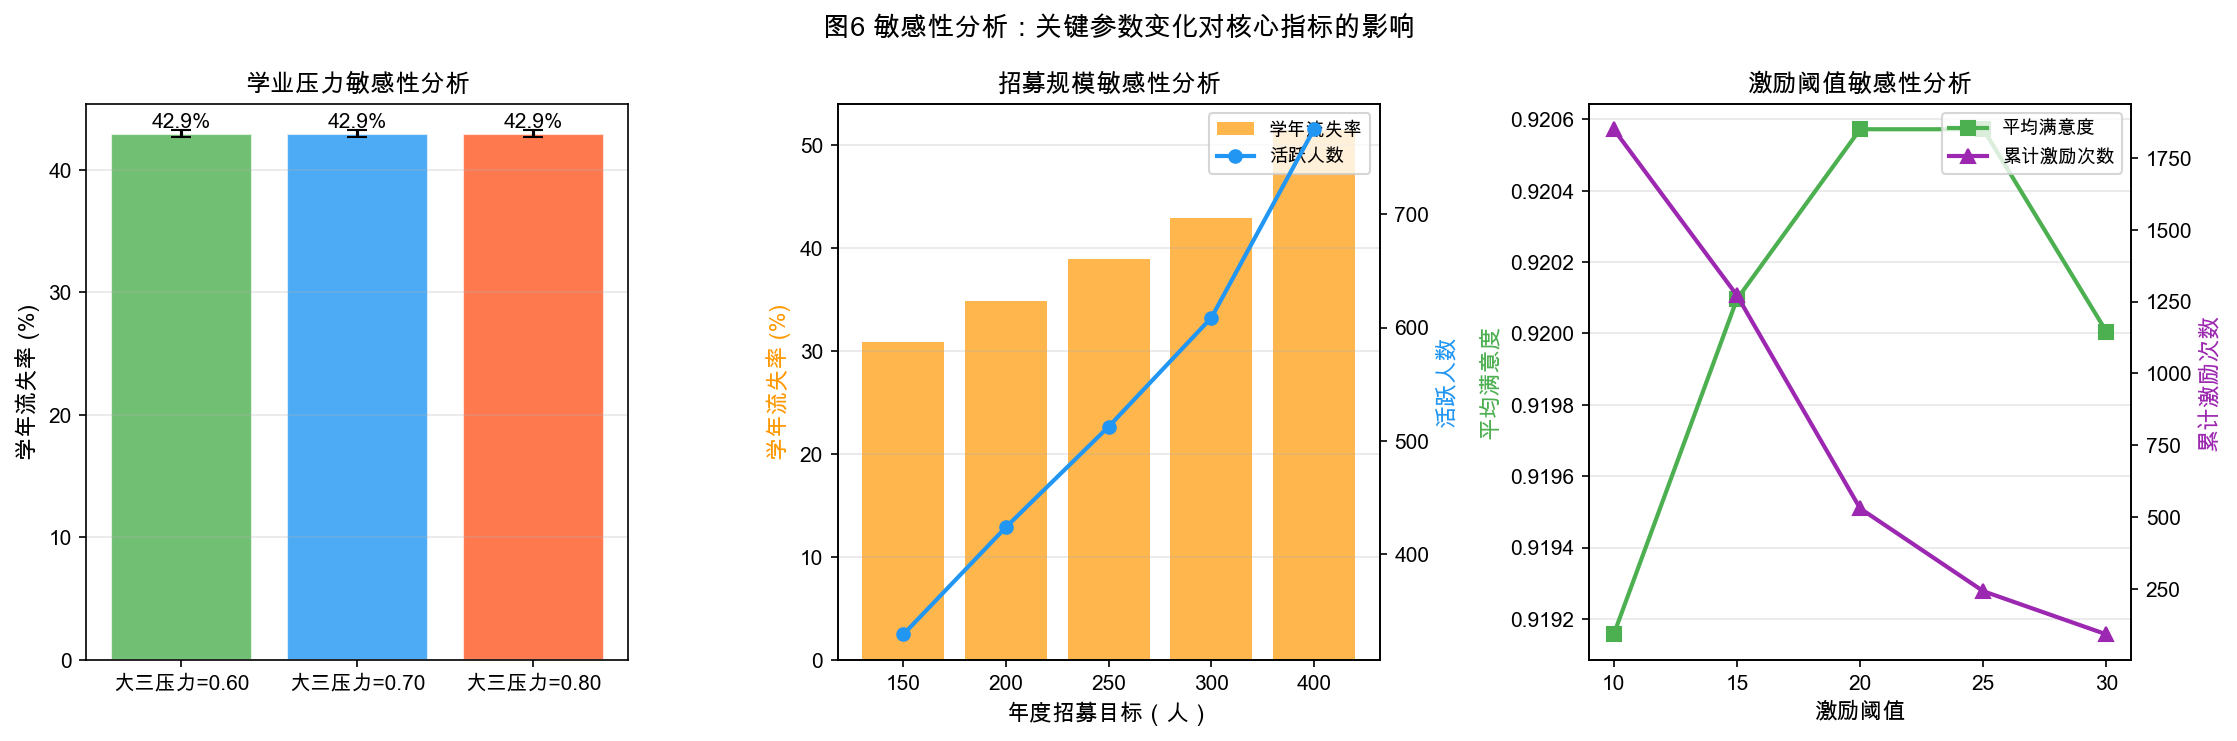
\includegraphics[width=0.85\textwidth,height=0.40\textheight]{../results/fig6_sensitivity}\par}
\vspace{0.5em}
(a) 学业压力参数升高$\pm10\%$对各实验流失率的影响；（b）激励区间参数变化对成员挫折感积累的调节效应。
\vspace{1em}
\end{figure}

本研究进行了两项稳健性检验。第一，年级4学业压力敏感性分析：将大四学业压力从0.80分别上调至0.90和0.95，考察其对各实验结果的影响。仿真结果显示，年级4学业压力变化对整体流失率的影响在$\pm 0.5\%$以内，结论未发生实质性改变。

第二，激励机制敏感性分析：改变激励下限（0.40—0.60）和激励上限（0.85—0.95），考察其对“强化激励”实验效应的影响。结果显示，激励区间宽度的变化对高服务量成员的挫折感积累速度有显著调节作用，支持了“激励存在非线性区间效应”的理论命题。

此外，本研究使用3次蒙特卡洛重复进行快速抽样验证（$n=3$），与正式15次重复结果的偏差在$\pm 1\%$以内，表明随机波动对核心结论的影响可控。

\section{讨论}

\subsection{行动与结构的互构机制}

本研究揭示了志愿服务场域中行动与结构互构的具体机制。在微观层面，学业压力、挫折感与满意度构成了成员流失的三条独立路径——学业压力反映了个体发展阶段的客观约束，挫折感反映了期望与现实之间的主观落差，满意度则连接了组织服务质量与个体持续意愿。在宏观层面，招募规模、届际制度与管理结构构成了场域的制度骨架——这些结构要素通过对个体激励的调节，间接决定了微观机制的强度与组合方式。

届际更替实验（exp1）的逆转模式为互构机制提供了有力例证。取消年级更替限制在短期内扩大了高年级志愿者池，降低了新生竞争压力，从而降低了流失率（结构改变→行动改善）。然而，这一改变同时弱化了管理层职位的稀缺性，减少了高年级成员的晋升激励，导致他们在后续年份中逐渐退出（结构改变通过改变激励结构，间接引发了新的流失——行动结果反向重塑了结构）。这一“短期改善、长期恶化”的模式提示，组织管理中的短期干预策略需要审慎评估其长期效应。

\subsection{管理启示}

本研究的政策实验结果为志愿服务组织管理提供了以下启示。第一，招募规模的控制是最具杠杆效应的单一干预手段。将年度招募目标从300人降至200人，可使流失率降低约20\%，同时提升晋升率7个百分点。这一结果的机制清晰：减少招募→降低竞争密度→提升高年级稀缺性与晋升概率→增强留任意愿。这提示组织在追求规模扩张的同时，应关注“有效规模”而非“名义规模”。

第二，激励政策应设计合理的区间结构，而非简单提高强度或降低门槛。本研究表明，激励存在下限（低于0.50时效果微弱）与上限（高于0.90时过载惩罚加速），提示组织应根据成员的服务阶段与服务量动态调整激励策略，而非采用单一门槛或线性递增设计。

第三，增加活动经费主要提升了活动质量（优秀项目占比从41.4\%升至69.2\%），而非直接降低流失率。这一结果提示，资源投入应与组织目标相匹配——如果主要目标是成员保留，应将资源用于改善服务体验而非单纯扩大活动规模。

\section{结论与局限}

本研究基于场域理论构建了志愿服务场域的多智能体仿真模型，识别了三机制独立驱动的成员流失格局，验证了招募规模、激励政策与届际制度对组织动态的差异化影响。主要结论如下：（1）学业压力与挫折感构成成员流失的双轨驱动机制，两者独立作用于流失概率；（2）减少招募规模是最具杠杆效应的单一干预手段，可使学年流失率降低约8.4个百分点；（3）激励政策呈现非线性区间效应，简单提高强度或降低门槛的边际效用有限；（4）取消届际更替限制呈现“短期改善、长期恶化”的逆转模式，反映了行动—结构互构的动态复杂性。

本研究存在若干局限。第一，样本代表性问题：数据来自北京高校志愿服务组织，研究结论不能直接外推至全国高校或其他类型的志愿服务组织。第二，数据质量限制：原始572条记录中存在大量精确重复记录（139种组合各重复约4次），可能源于数据录入过程，去重后的样本量（137条唯一记录）较小，影响了统计检验力。第三，模型抽象性：ABM不可避免地对现实进行了抽象简化，组织文化、同伴网络效应等重要因素尚未纳入模型。第四，年级效应的不稳定性：逻辑回归中高年级变量的显著性在去重后消失，提示年级抑制的具体机制有待进一步检验。

未来研究可从以下方向拓展：（1）整合同伴网络效应，构建多层场的互构模型；（2）利用纵向追踪数据校准流失机制的时间动态；（3）在多组织样本上验证政策实验结论的外部有效性；（4）探索ABM与真实世界实验相结合的准实验设计路径。

\vspace{2em}
\bibliographystyle{apalike}
\bibliography{refs}
